\documentclass{article}
\usepackage[english, greek, main=greek]{babel}
\usepackage[utf8x]{inputenc}
\usepackage[unicode]{hyperref}
\usepackage{listings}
\usepackage{color}
\usepackage{float}
\usepackage{caption}
\usepackage{subcaption}
\usepackage[export]{adjustbox}
\usepackage{amsmath,amsthm,mathtools}
\usepackage{cleveref}
\hypersetup{pdfborder=0 0 0}
\addto\captionsgreek{
    \crefname{figure}{Σχήμα.}{Σχήματα.}
    \Crefname{figure}{Σχήμα.}{Σχήματα.}
}


\begin{document}

\begin{titlepage}
    \begin{center}
        \vspace*{1cm}
            
        \Huge
        \textbf{Υπολογιστική Εργασία στο \foreignlanguage{english}{IBM SPSS}}
            
        \vspace{0.5cm}
        \LARGE
        \textbf{Ανάλυση Δεδομένων Ημερήσιας Θνητότητας στην Μολδαβία και το Ηνωμένο Βασίλειο}
            
        \vspace{1.5cm}
            
        Τσαμουρίδης Αναστάσιος Αθανάσιος \\
            
        \vfill
            
        \Large
        Ιούλιος 2021, 4\textsuperscript{ο} Εξάμηνο \\
        Τμήμα Ηλεκτρολόγων Μηχανικών και Μηχανικών Υπολογιστών\\
        Αριστοτέλειο Πανεπιστήμιο Θεσσαλονίκης\\
        
    \end{center}
\end{titlepage}

\author{}
\date{}

\newpage

\tableofcontents

\newpage
\section{Εισαγωγή}

    Στο παρόν έγγραφο, γίνεται ανάλυση της θνητότητας στις χώρες της Μολδαβίας και του Ηνωμένου Βασιλείου και τα στατιστικά των δύο χωρών συγκρίνονται. 
    
\section{Συλλογή δεδομένων}

    Για την ανάλυση του ποσοστού θνητότητας της νόσου \foreignlanguage{english}{Covid-19} επιλέχτηκαν στατιστικά δεδομένα από την Μολδαβία και το Ηνωμένο Βασίλειο. Τα δεδομένα των δύο χωρών αναφέρονται, συχνά, ως δείγμα Α και δείγμα Β, αντίστοιχα. Τα δεδομένα που χρησιμοποιούνται προέρχονται από το:\newline
    \href{https://www.worldometers.info/coronavirus/}{\foreignlanguage{english}{https://www.worldometers.info/coronavirus/}}.

    \subsection{Επιλογή δείγματος}
     \label{sec:sample}
        Για τις δύο χώρες επιλέχτηκε ένα δείγμα μεγέθους 45 ημερών (ένας και μισός μήνας, θεωρώντας ότι ο μήνας έχει, κατά μέσο όρο, 30 ημέρες). Ως αρχή του δείγματος για τους καθημερινούς θανάτους επιλέχτηκε η κορύφωση του κύματος για το 2021. Ομοίως, για τα ημερήσια κρούσματα. Συγκεκριμένα:
        \begin{enumerate}
        \item Για την Μολδαβία:
            \begin{itemize}
                \item Ως πρώτη ημέρα για την καταγραφή ημερήσιων κρουσμάτων ορίζεται η 24\textsuperscript{η} Μαρτίου (22073 κρούσματα). 
                \item Ως πρώτη ημέρα για την καταγραφή ημερήσιων θανάτων ορίζεται η 30\textsuperscript{η} Μαρτίου (46 θάνατοι). Εδώ πρέπει να σημειωθεί ότι ο ίδιος αριθμός ημερήσιων θανάτων παρουσιάστηκε και στις 6 Απριλίου, ωστόσο επιλέχτηκε ως κορύφωση η πρώτη εμφάνιση του μεγίστου αριθμού θανάτων.
            \end{itemize}
        \item Για το Ηνωμένο Βασίλειο:
            \begin{itemize}
                \item Ως πρώτη ημέρα για την καταγραφή των ημερήσιων κρουσμάτων ορίζεται η 8\textsuperscript{η} ημέρα του Ιανουαρίου (67803 κρούσματα). 
                \item Ως πρώτη ημέρα για την καταγραφή ημερήσιων θανάτων ορίζεται η 20\textsuperscript{η} Ιανουαρίου (1823 θάνατοι).
            \end{itemize}
        \end{enumerate}
        
        Για τις δύο χώρες, στα δεδομένα δεν εμφανίζεται κάποια προβληματική ή ακραία τιμή. Στον \autoref{Moldova_data} και στον \autoref{UK_data} παρατίθενται τα δεδομένα που συλλέχθησαν.
                
        \begin{table} 
            \centering
            \caption{Δεδομένα Μολδαβίας}
            \label{Moldova_data}
            \resizebox{.6\textheight}{!}{%
            \begin{tabular}{|c|c|c|c|c|}
                Ημ. Κρουσμάτων & Κρούσματα & Ημ. Θανάτων & Θάνατοι & Ποσοστό Θνητότητας \\ \hline
                24-Μαρ-21 & 2273 & 30-Μαρ-21 & 46 & 2,023757 \\ \hline
                25-Μαρ-21 & 2132 & 31-Μαρ-21 & 45 & 2,110694 \\ \hline
                26-Μαρ-21 & 1866 & 1-Απρ-21 & 43 & 2,304394 \\ \hline
                27-Μαρ-21 & 1674 & 2-Απρ-21 & 45 & 2,688172 \\ \hline
                28-Μαρ-21 & 861 & 3-Απρ-21 & 44 & 5,110337 \\ \hline
                29-Μαρ-21 & 932 & 4-Απρ-21 & 44 & 4,72103 \\ \hline
                30-Μαρ-21 & 917 & 5-Απρ-21 & 42 & 4,580153 \\ \hline
                31-Μαρ-21 & 1871 & 6-Απρ-21 & 46 & 2,458578 \\ \hline
                1-Απρ-21 & 1515 & 7-Απρ-21 & 44 & 2,90429 \\ \hline
                2-Απρ-21 & 1380 & 8-Απρ-21 & 39 & 2,826087 \\ \hline
                3-Απρ-21 & 1258 & 9-Απρ-21 & 32 & 2,54372 \\ \hline
                4-Απρ-21 & 693 & 10-Απρ-21 & 30 & 4,329004 \\ \hline
                5-Απρ-21 & 703 & 11-Απρ-21 & 19 & 2,702703 \\ \hline
                6-Απρ-21 & 773 & 12-Απρ-21 & 21 & 2,716688 \\ \hline
                7-Απρ-21 & 1155 & 13-Απρ-21 & 29 & 2,510823 \\ \hline
                8-Απρ-21 & 1428 & 14-Απρ-21 & 28 & 1,960784 \\ \hline
                9-Απρ-21 & 910 & 15-Απρ-21 & 27 & 2,967033 \\ \hline
                10-Απρ-21 & 830 & 16-Απρ-21 & 28 & 3,373494 \\ \hline
                11-Απρ-21 & 331 & 17-Απρ-21 & 27 & 8,1571 \\ \hline
                12-Απρ-21 & 603 & 18-Απρ-21 & 23 & 3,814262 \\ \hline
                13-Απρ-21 & 544 & 19-Απρ-21 & 20 & 3,676471 \\ \hline
                14-Απρ-21 & 1001 & 20-Απρ-21 & 25 & 2,497502 \\ \hline
                15-Απρ-21 & 812 & 21-Απρ-21 & 27 & 3,325123 \\ \hline
                16-Απρ-21 & 698 & 22-Απρ-21 & 25 & 3,581662 \\ \hline
                17-Απρ-21 & 628 & 23-Απρ-21 & 23 & 3,66242 \\ \hline
                18-Απρ-21 & 403 & 24-Απρ-21 & 18 & 4,466501 \\ \hline
                19-Απρ-21 & 341 & 25-Απρ-21 & 21 & 6,158358 \\ \hline
                20-Απρ-21 & 453 & 26-Απρ-21 & 15 & 3,311258 \\ \hline
                21-Απρ-21 & 700 & 27-Απρ-21 & 17 & 2,428571 \\ \hline
                22-Απρ-21 & 618 & 28-Απρ-21 & 18 & 2,912621 \\ \hline
                23-Απρ-21 & 509 & 29-Απρ-21 & 15 & 2,946955 \\ \hline
                24-Απρ-21 & 380 & 30-Απρ-21 & 17 & 4,473684 \\ \hline
                25-Απρ-21 & 241 & 01-Μάιος-2021 & 14 & 5,809129 \\ \hline
                26-Απρ-21 & 246 & 02-Μάιος-2021 & 12 & 4,878049 \\ \hline
                27-Απρ-21 & 329 & 03-Μάιος-2021 & 12 & 3,647416 \\ \hline
                28-Απρ-21 & 424 & 04-Μάιος-2021 & 19 & 4,481132 \\ \hline
                29-Απρ-21 & 370 & 05-Μάιος-2021 & 23 & 6,216216 \\ \hline
                30-Απρ-21 & 329 & 06-Μάιος-2021 & 20 & 6,079027 \\ \hline
                01-Μάιος-2021 & 323 & 07-Μάιος-2021 & 17 & 5,263158 \\ \hline
                02-Μάιος-2021 & 175 & 08-Μάιος-2021 & 14 & 8 \\ \hline
                03-Μάιος-2021 & 43 & 09-Μάιος-2021 & 9 & 20,930233 \\ \hline
                04-Μάιος-2021 & 126 & 10-Μάιος-2021 & 6 & 4,761905 \\ \hline
                05-Μάιος-2021 & 316 & 11-Μάιος-2021 & 12 & 3,797468 \\ \hline
                06-Μάιος-2021 & 333 & 12-Μάιος-2021 & 11 & 3,303303 \\ \hline
                07-Μάιος-2021 & 260 & 13-Μάιος-2021 & 14 & 5,384615 \\ \hline
            \end{tabular}%
            }
        \end{table}
        
        \begin{table}{\textheight = 25cm}
            \centering
            \caption{Δεδομένα Ηνωμένου Βασιλείου}
            \label{UK_data}
            \resizebox{.6\textheight}{!}{%
            \begin{tabular}{|c|c|c|c|c|}
                Ημ. Κρουσμάτων & Κρούσματα & Ημ. Θανάτων & Θάνατοι & Ποσοστό Θνητότητας \\ \hline
                8-Ιαν-21 & 67803 & 20-Ιαν-21 & 1823 & 2,688672 \\ \hline
                9-Ιαν-21 & 59717 & 21-Ιαν-21 & 1292 & 2,163538 \\ \hline
                10-Ιαν-21 & 54739 & 22-Ιαν-21 & 1403 & 2,563072 \\ \hline
                11-Ιαν-21 & 45999 & 23-Ιαν-21 & 1350 & 2,934846 \\ \hline
                12-Ιαν-21 & 45364 & 24-Ιαν-21 & 611 & 1,346883 \\ \hline
                13-Ιαν-21 & 47350 & 25-Ιαν-21 & 593 & 1,252376 \\ \hline
                14-Ιαν-21 & 48502 & 26-Ιαν-21 & 1633 & 3,366871 \\ \hline
                15-Ιαν-21 & 55553 & 27-Ιαν-21 & 1728 & 3,110543 \\ \hline
                16-Ιαν-21 & 41192 & 28-Ιαν-21 & 1241 & 3,012721 \\ \hline
                17-Ιαν-21 & 38455 & 29-Ιαν-21 & 1247 & 3,242751 \\ \hline
                18-Ιαν-21 & 37395 & 30-Ιαν-21 & 1202 & 3,214333 \\ \hline
                19-Ιαν-21 & 33235 & 31-Ιαν-21 & 588 & 1,769219 \\ \hline
                20-Ιαν-21 & 38726 & 1-Φεβ-21 & 407 & 1,050974 \\ \hline
                21-Ιαν-21 & 37752 & 2-Φεβ-21 & 1451 & 3,843505 \\ \hline
                22-Ιαν-21 & 40111 & 3-Φεβ-21 & 1324 & 3,30084 \\ \hline
                23-Ιαν-21 & 33431 & 4-Φεβ-21 & 916 & 2,739972 \\ \hline
                24-Ιαν-21 & 29897 & 5-Φεβ-21 & 1015 & 3,394989 \\ \hline
                25-Ιαν-21 & 22112 & 6-Φεβ-21 & 829 & 3,749096 \\ \hline
                26-Ιαν-21 & 20016 & 7-Φεβ-21 & 374 & 1,868505 \\ \hline
                27-Ιαν-21 & 25217 & 8-Φεβ-21 & 333 & 1,320538 \\ \hline
                28-Ιαν-21 & 28627 & 9-Φεβ-21 & 1054 & 3,681839 \\ \hline
                29-Ιαν-21 & 28910 & 10-Φεβ-21 & 1002 & 3,465929 \\ \hline
                30-Ιαν-21 & 23138 & 11-Φεβ-21 & 679 & 2,934567 \\ \hline
                31-Ιαν-21 & 20964 & 12-Φεβ-21 & 759 & 3,620492 \\ \hline
                1-Φεβ-21 & 18495 & 13-Φεβ-21 & 622 & 3,363071 \\ \hline
                2-Φεβ-21 & 16738 & 14-Φεβ-21 & 258 & 1,541403 \\ \hline
                3-Φεβ-21 & 19088 & 15-Φεβ-21 & 230 & 1,204946 \\ \hline
                4-Φεβ-21 & 20513 & 16-Φεβ-21 & 800 & 3,899966 \\ \hline
                5-Φεβ-21 & 19000 & 17-Φεβ-21 & 739 & 3,889474 \\ \hline
                6-Φεβ-21 & 18153 & 18-Φεβ-21 & 455 & 2,506473 \\ \hline
                7-Φεβ-21 & 15754 & 19-Φεβ-21 & 534 & 3,389615 \\ \hline
                8-Φεβ-21 & 14022 & 20-Φεβ-21 & 446 & 3,180716 \\ \hline
                9-Φεβ-21 & 12292 & 21-Φεβ-21 & 214 & 1,74097 \\ \hline
                10-Φεβ-21 & 12938 & 22-Φεβ-21 & 178 & 1,375792 \\ \hline
                11-Φεβ-21 & 13417 & 23-Φεβ-21 & 549 & 4,091824 \\ \hline
                12-Φεβ-21 & 15056 & 24-Φεβ-21 & 443 & 2,942349 \\ \hline
                13-Φεβ-21 & 13233 & 25-Φεβ-21 & 323 & 2,440868 \\ \hline
                14-Φεβ-21 & 10908 & 26-Φεβ-21 & 346 & 3,171984 \\ \hline
                15-Φεβ-21 & 9708 & 27-Φεβ-21 & 290 & 2,987227 \\ \hline
                16-Φεβ-21 & 10561 & 28-Φεβ-21 & 144 & 1,363507 \\ \hline
                17-Φεβ-21 & 12646 & 1-Μαρ-21 & 104 & 0,822394 \\ \hline
                18-Φεβ-21 & 11988 & 2-Μαρ-21 & 343 & 2,861195 \\ \hline
                19-Φεβ-21 & 11958 & 3-Μαρ-21 & 315 & 2,63422 \\ \hline
                20-Φεβ-21 & 10346 & 4-Μαρ-21 & 242 & 2,339068 \\ \hline
                21-Φεβ-21 & 9777 & 5-Μαρ-21 & 236 & 2,413828 \\ \hline
            \end{tabular}%
            }
        \end{table}

\newpage

Στο \autoref{all} παρατίθενται τα γραφήματα όλων των ημερήσιων κρουσμάτων και θανάτων για τις δύο χώρες, όπως αυτές εμφανίζονται στο \newline \href{https://www.worldometers.info/coronavirus/}{\foreignlanguage{english}{https://www.worldometers.info/coronavirus/}}.

\vfill
\begin{figure}[H]
    \centering
    \begin{subfigure}[b]{0.475\textwidth}
        \centering
        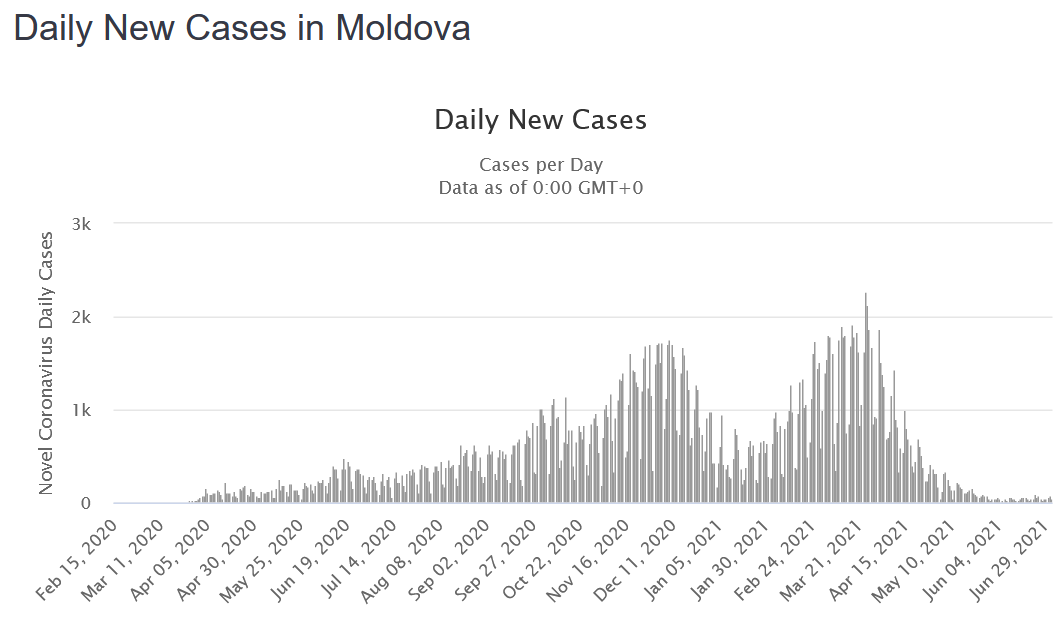
\includegraphics[width=\textwidth]{media/3/moldova_cases.png}
        \caption{Κρούσματα Μολδαβίας}    
    \end{subfigure}
    \hfill
    \begin{subfigure}[b]{0.475\textwidth}  
        \centering 
        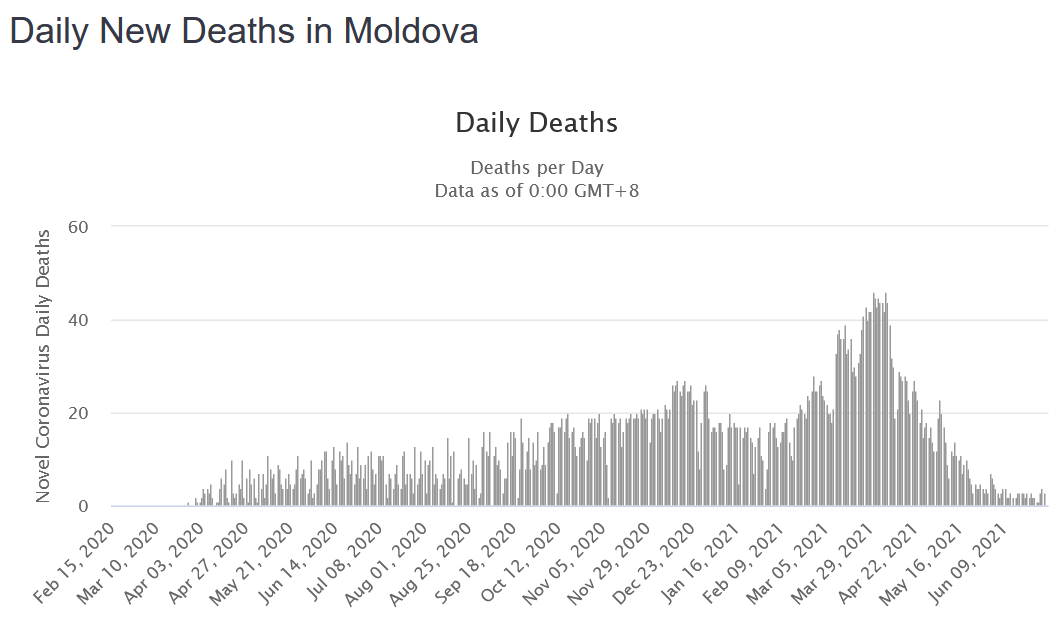
\includegraphics[width=\textwidth]{media/3/moldova_deaths.png}
        \caption{Θάνατοι Μολδαβίας}    
    \end{subfigure}
    \vskip\baselineskip
    \begin{subfigure}[b]{0.475\textwidth}   
        \centering 
        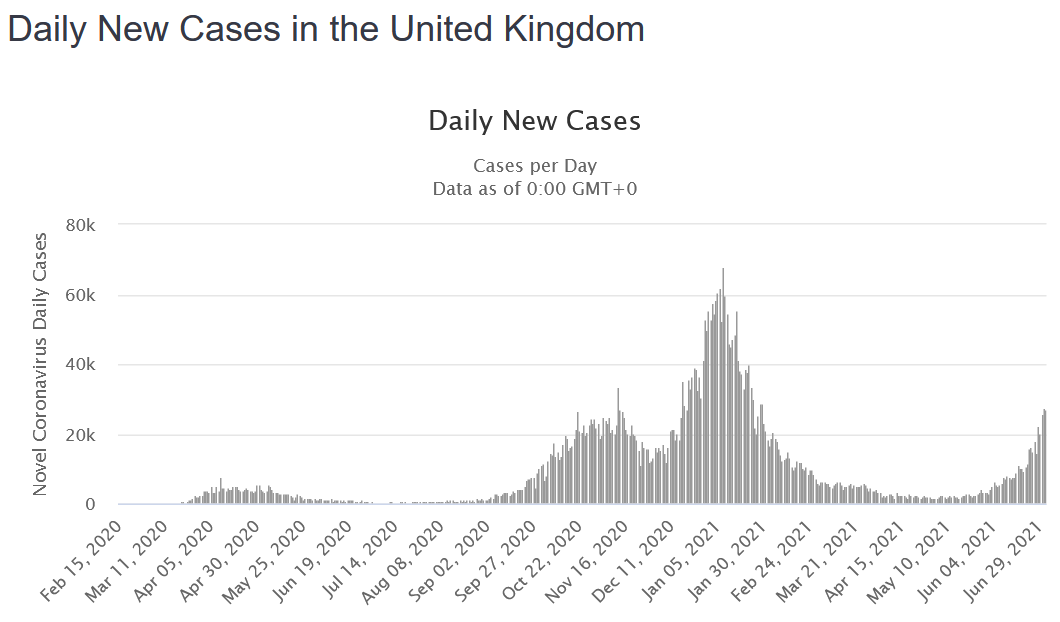
\includegraphics[width=\textwidth]{media/3/UK_cases.png}
        \caption{Κρούσματα Ηνωμένου Βασιλείου}  
    \end{subfigure}
    \hfill
    \begin{subfigure}[b]{0.475\textwidth}   
        \centering 
        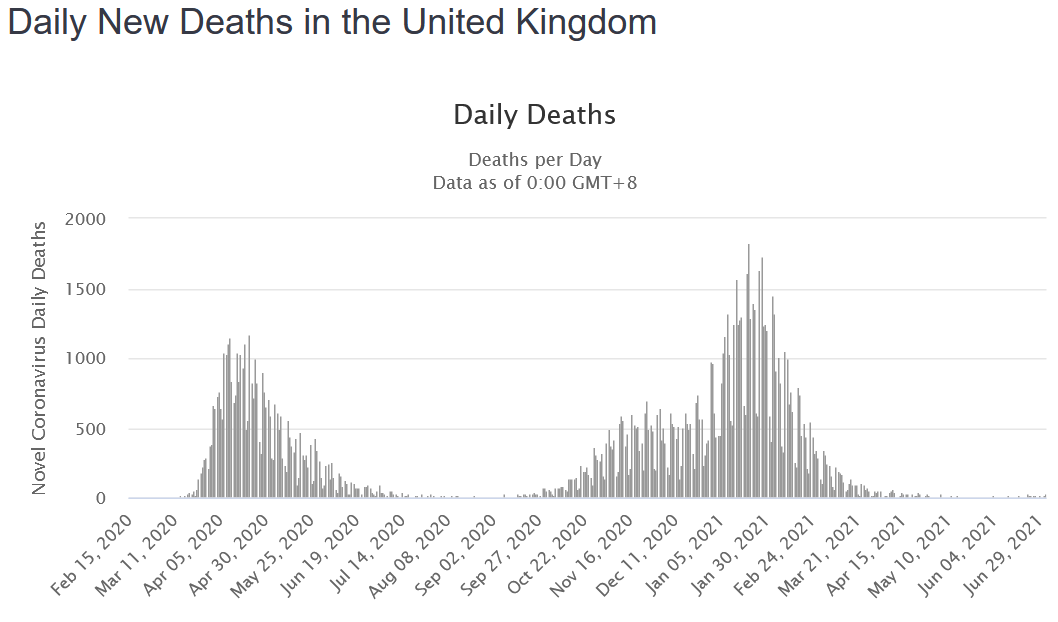
\includegraphics[width=\textwidth]{media/3/UK_deaths.png}
        \caption{Θάνατοι Ηνωμένου Βασιλείου}
    \end{subfigure}
    \caption{Ημερήσια Κρούσματα και Ημερήσιοι Θάνατοι στην Μολδαβία και το Ηνωμένο Βασίλειο, όπως αυτά εμφανίζονται στο \foreignlanguage{english}{worldometers.info}}
    \label{all}
\end{figure}
\vfill
\newpage

\section{Μελέτη Α}

\emph{Μελέτη της κατανομής και της Μέσης Τιμής του Ημερήσιου Ποσοστού Θνητότητας στις δύο Χώρες την Περίοδο μετά την Κορύφωση του Κύματος Κορωνοϊού.} 

\subsection{Σχολιασμός της Κατανομής του Ημερήσιου Ποσοστού Θνητότητας}

    Αρχικά, παραθέτουμε το \autoref{Stats}, στο οποίο παρουσιάζονται τα βασικά μέτρα κεντρικής τάσης και μεταβλητότητας για τα ποσοστά θνητότητας στις δύο χώρες.
    
    \begin{figure}[H]
        \centering
    	\begin{adjustbox}{center}
    		\begin{subfigure}[c]{1\textwidth}    
    			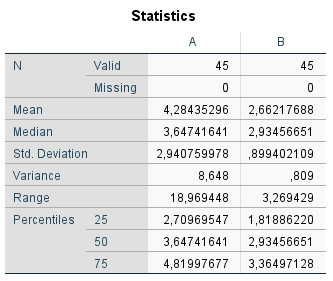
\includegraphics[width=1\textwidth,height=\textheight,keepaspectratio]{media/2/stats.png}
    		\end{subfigure}%
    	\end{adjustbox}
    	\caption{Βασικά Μέτρα Κεντρικής Τάσης και Μεταβλητότητας για τα ποσοστά θνητότητας στην Μολδαβία και το Ηνωμένο Βασίλειο}
        \label{Stats}
    \end{figure}
    
    Όπως βλέπουμε, ο μέσος όρος και η διάμεσος της θνητότητας εμφανίζονται μεγαλύτερα για την χώρα της Μολδαβίας, υποδηλώνοντας ότι μεγαλύτερο ποσοστό κρουσμάτων οδηγήθηκαν στον θάνατο, σε σύγκριση με την Μεγάλη Βρετανία. Το ίδιο συμβαίνει με τα μέτρα μεταβλητότητας, κάτι που δείχνει μεγαλύτερη μεταβολή των ποσοστών θνητότητας στην Μολδαβία.
    
    Στο \autoref{Histograms} παρατίθενται τα ιστογράμματα θνητότητας των δύο χωρών και σημειώνεται και η μορφή της κανονικής κατανομής
    
    \begin{figure}[H]
    
        \centering	
    	\begin{adjustbox}{center}
            \begin{subfigure}[c]{.8\textwidth}
    			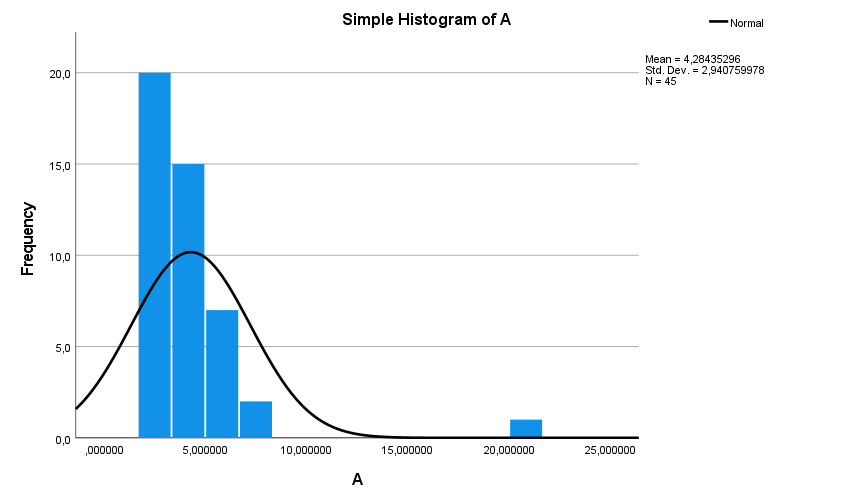
\includegraphics[width=1\textwidth,height=\textheight,keepaspectratio]{media/2/histA.png}
    		\end{subfigure}
    
    		\begin{subfigure}[c]{.8\textwidth}    
    			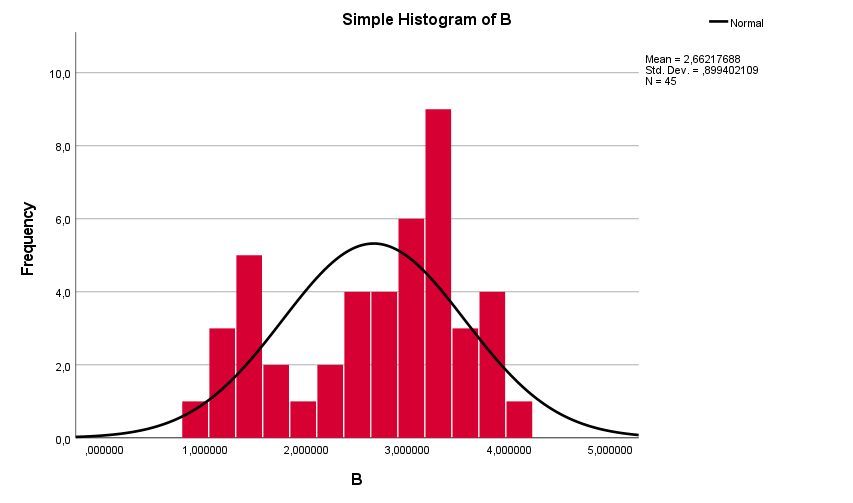
\includegraphics[width=1\textwidth,height=\textheight,keepaspectratio]{media/2/histB.png}
    		\end{subfigure}%		
    	\end{adjustbox}
    	\caption{Ιστογράμματα ποσοστού θνητότητας στην Μολδαβία και την Μεγάλη Βρετανία}
    	\label{Histograms}
    \end{figure}
    
    Στο ιστόγραμμα του δείγματος Α φαίνεται να έχουμε συγκέντρωση των ποσοστών θνητότητας σε μικρότερες τιμές. Αντίθετα στο δείγμα Β, το ιστόγραμμα δείχνει να πλησιάζει περισσότερο την κανονική κατανομή.
    
    Σχηματίζουμε τα θηκογράμματα για τα δεδομένα για να εξετάσουμε καλύτερα την κατανομή που ακολουθούν τα δείγματα Α και Β. Στο \autoref{boxplot_all} φαίνονται τα θηκογράμματα και για τα δύο δείγματα. Για λόγους ευκρίνειας, παραθέτουμε και τα θηκογράμματα σε ξεχωριστή κλίμακα στο \autoref{boxplot_separate}.
    
    \begin{figure}[H]
        \centering
    	\begin{adjustbox}{center}
    		\begin{subfigure}[c]{1\textwidth}    
    			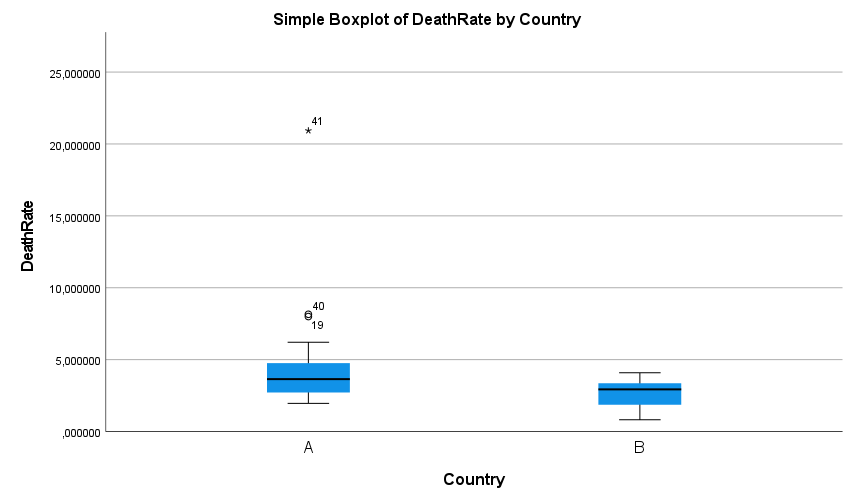
\includegraphics[width=1\textwidth,height=\textheight,keepaspectratio]{media/2/boxplot_together.png}
    		\end{subfigure}%
    	\end{adjustbox}
    	\caption{Θηκογράμματα Ποσοστών Θνητότητας στην Μολδαβία και την Μεγάλη Βρετανία}
        \label{boxplot_all}
    \end{figure}
    
    \begin{figure}[H]
    
        \centering	
    	\begin{adjustbox}{center}
            \begin{subfigure}[c]{.7\textwidth}
    			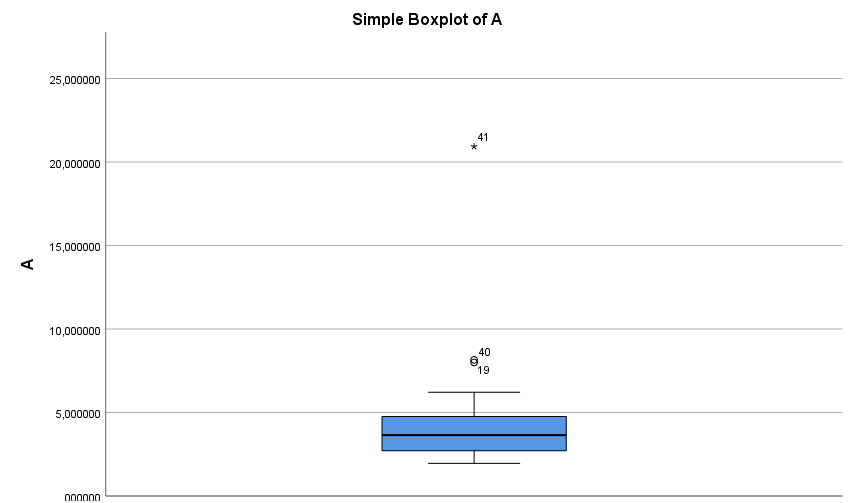
\includegraphics[width=1\textwidth,height=\textheight,keepaspectratio]{media/2/boxplotA.png}
    		\end{subfigure}
    
    		\begin{subfigure}[c]{.7\textwidth}    
    			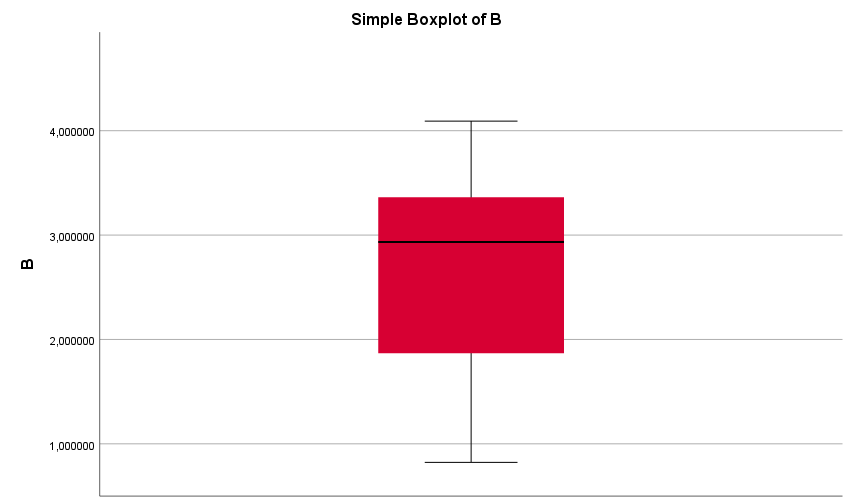
\includegraphics[width=1\textwidth,height=\textheight,keepaspectratio]{media/2/boxplotB.png}
    		\end{subfigure}%		
    	\end{adjustbox}
    	\caption{Θηκογράμματα Ποσοστών Θνητότητας στην Μολδαβία και την Μεγάλη Βρετανία σε Ξεχωριστή Κλίμακα}
    	\label{boxplot_separate}
    \end{figure}
    
    Από τα παραπάνω σχήματα, μπορούμε να εξάγουμε τα εξής συμπεράσματα:
    \begin{enumerate}
              \item Για την Μολδαβία (Δείγμα Α):
                \begin{itemize}
                  \item Η διάμεσος βρίσκεται περίπου στο μέσον των \foreignlanguage{english}{Q\textsubscript{1}} και \foreignlanguage{english}{Q\textsubscript{3}}, αν και τείνει να πλησιάζει το πρώτο τεταρτομόριο.
                  \item Οι μύστακες φαίνεται να έχουν το ίδιο μήκος.
                  \item Ωστόσο, σημειώνονται τρεις ακραίες τιμές.
                \end{itemize}
                Συνεπώς, για το δείγμα Α, δεν μπορούμε να αποδεχτούμε ότι ακολουθεί κανονική κατανομή.
              \item Για το Ηνωμένο Βασίλειο (Δείγμα Β):
              \begin{itemize}
                  \item Οι μύστακες έχουν σχεδόν το ίδιο μήκος.
                  \item Η διάμεσος πλησιάζει ελάχιστα περισσότερο στο \foreignlanguage{english}{Q\textsubscript{3}}. Ωστόσο, επειδή το δείγμα είναι σχετικά μικρό (45 τιμές) μπορούμε να αποδεχτούμε ότι βρίσκεται στο μέσον του ενδοτεταρτομοριακού εύρους.
                  \item Δεν υπάρχουν ακραίες τιμές στο δείγμα.
              \end{itemize}
                  Επομένως, μπορούμε να αποδεχτούμε την κανονική κατανομή ως την κατανομή του δείγματος Β.
            \end{enumerate}
    
    \subsection{Μελέτη της Μέσης Τιμής του Ημερήσιου Ποσοστού Θνητότητας}
    
    \emph{Σε αυτό το εδάφιο θα γίνει μελέτη της μέσης τιμής των δύο δειγμάτων. Παράλληλα θα εξεταστεί για διάστημα εμπιστοσύνης 95\% της μέσης τιμής αν η θνητότητα δύναται να φτάσει το 5\%}.
    
    Στο Σχήμα \autoref{mean} σημειώνονται τα αποτελέσματα για διάστημα εμπιστοσύνης 95\% της μέσης τιμής. 
    
    \begin{figure}[t]
      \centering
        \begin{subfigure}{0.8\linewidth}
        \centering
          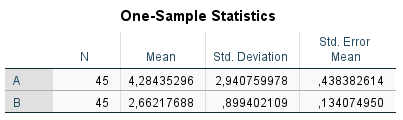
\includegraphics[width=\linewidth]{media/2/one_sample_statistics.png}
        \end{subfigure}\\
        \begin{subfigure}{1\linewidth}
            \centering
          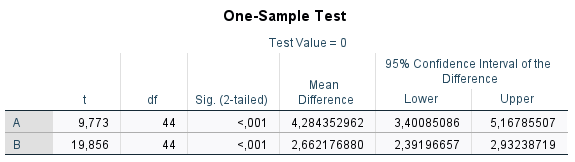
\includegraphics[width=\linewidth]{media/2/de.png}
        \end{subfigure}
      \caption{Αποτελέσματα Ανάλυσης για 95\% Διάστημα Εμπιστοσύνης για την Μέση τιμή της Θνητότητας σε Μολδαβία και Μεγάλη Βρετανία}
      \label{mean}
    \end{figure}

     Όπως προκύπτει από τα παραπάνω, το διάστημα εμπιστοσύνης προκύπτει ίσο με $ [3.40085086, 5.16785507] $ για το δείγμα Α και $ [2.39196657, 2.93238719] $ για το δείγμα Β. Παρατηρούμε ότι το εύρος του διαστήματος εμπιστοσύνης για την Μεγάλη Βρετανία είναι μικρότερο σε σύγκριση με αυτό της Μολδαβίας. Επίσης, αξίζει να σημειωθεί ότι το διάστημα εμπιστοσύνης της Μολδαβίας εμφανίζει μεγαλύτερες τιμές από αυτό του δείγματος Β, επιβεβαιώνοντας τα όσα ειπώθηκαν έως τώρα.
     
     Η μέση τιμή της θνητότητας μπορεί να φτάσει το 5\% για την Μολδαβία, όχι όμως και για την Αγγλία. Αυτό προκύπτει εύκολα παρατηρώντας αν ανήκει, ή όχι, το 5 στο διάστημα εμπιστοσύνης κάθε δείγματος. Στο \autoref{percent5} επιβεβαιώνονται τα παραπάνω χρησιμοποιώντας ως \foreignlanguage{english}{Test Value} το 5. Όπως βλέπουμε προκύπτουν τα διαστήματα  $ [-1.59914914, 0.16788507] $ για το δείγμα Α (στο οποίο ανήκει το μηδέν) και $ [-2.60803343, -2.06761281] $ για το δείγμα Β (στο οποίο δεν ανήκει το μηδέν).
     
         \begin{figure}[H]
        \centering
    	\begin{adjustbox}{center}
    		\begin{subfigure}[c]{1\textwidth}    
    			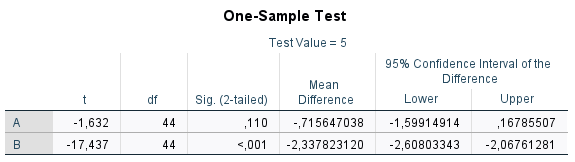
\includegraphics[width=1\textwidth,height=\textheight,keepaspectratio]{media/2/percent5.png}
    		\end{subfigure}%
    	\end{adjustbox}
    	\caption{Διάστημα εμπιστοσύνης 95\% για την Μέση τιμή της Θνητότητας σε Μολδαβία και Μεγάλη Βρετανία με \foreignlanguage{english}{Test Value} 5}
        \label{percent5}
    \end{figure}
     
     \newpage
     
     Τα παραπάνω ισχύουν με μία μικρή επιφύλαξη, καθώς το διάστημα εμπιστοσύνης είναι στο 95\% (όχι 100\%) και το δείγμα σχετικά μεκρό, οπότε δεν μπορούμε να είμαστε απόλυτα βέβαιοι για τα αποτελέσματα μας.
    
\subsection{Σύγκριση της Μέσης Τιμής του Ημερήσιου Ποσοστού Θνητότητας}
    
     \emph{Σε αυτό το εδάφιο θα εξεταστεί αν η μέση τιμή του ποσοστού θνητότητας μπορεί να είναι ίδια για την 
     Μολδαβία και το Ηνωμένο Βασίλειο.}
     
     Μελετώντας το 95\% διάστημα εμπιστοσύνης για το μ\textsubscript{A} - μ\textsubscript{Β} προκύπτουν τα αποτελέσματα που εμφανίζονται στο \autoref{m1_m2_dif}.
    
   \begin{figure}[H]
      \centering
        \begin{subfigure}{0.8\linewidth}
        \centering
          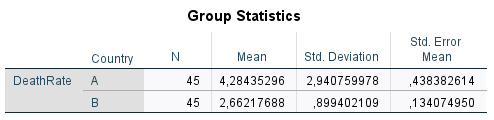
\includegraphics[width=\linewidth]{media/2/means_comparison1.png}
        \end{subfigure}\\
        \begin{subfigure}{1\linewidth}
            \centering
          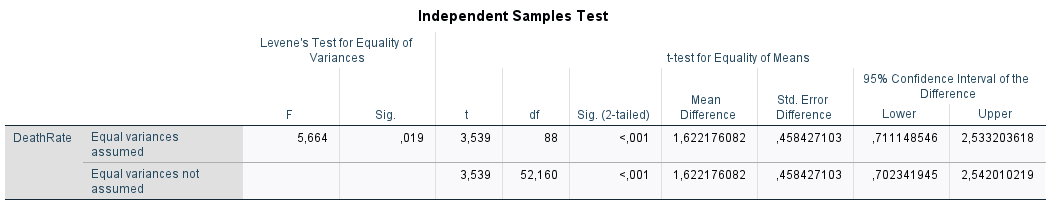
\includegraphics[width=\linewidth]{media/2/means_comparison2.png}
        \end{subfigure}
      \caption{Αποτελέσματα Ανάλυσης για 95\% Διάστημα Εμπιστοσύνης για την Διαφορά των Μέσων Τιμών της Θνητότητας σε Μολδαβία και Μεγάλη Βρετανία}
      \label{m1_m2_dif}
    \end{figure}
     
     Όπως φαίνεται απο τον πρώτο πίνακα οι τυπικές αποκλίσεις, άρα και οι διακυμάνσεις των δύο δειγμάτων, δεν μπορούν να θεωρηθούν ίσες.
     
     Από τον δεύτερο πίνακα βλέπουμε ότι το 95\% διάστημα εμπίστοσύνης για το μ\textsubscript{A} - μ\textsubscript{Β} προκύπτει ως:
     \begin{itemize}
       \item $ [0.711148546, 2.533203618] $ αν θεωρήσουμε ότι οι διακυμάνσεις των δύο δειγμάτων είναι ίσες.
       \item $ [0.702341945, 2.542010219] $ αν θεωρήσουμε ότι οι διακυμάνσεις των δύο δειγμάτων δεν είναι ίσες, κάτι που ισχύει στην περίπτωση μας.
     \end{itemize}
     
     Σε κάθε μία από τις παραπάνω περιπτώσεις, το διάστημα εμπιστοσύνης δεν περιέχει την μηδενική τιμή, συνεπώς, η μέση τιμή του ημερήσιου ποσοστού θανάτων δεν μπορεί να είναι ίδια για τις δύο χώρες. Επιπρόσθετα, το διάστημα έχει θετικές τιμές, κάτι που υποδηλώνει ότι η μέση τιμή του δείγματος Α είναι μεγαλύτερη από την μέση τιμή του δείγματος Β. Εδώ πρέπει να σημειωθεί πως τα δείγματα είναι σχετικά μικρά, και το διάστημα εμπιστοσύνης ίσο με 95\%, οπότε δεν μπορούμε να είμαστε απολύτως βέβαιοι ότι τα παραπάνω αποτελέσματα είναι απολύτως ακριβή.
    
\newpage
    
\section{Μελέτη Β}
\emph{Σε αυτή την μελέτη εξετάζεται η συσχέτιση των ημερήσιων κρουσμάτων με τον χρόνο μετά την κορύφωση του κύματος} 

    \subsection{Συσχέτιση Ημερήσιων Κρουσμάτων και Θανάτων με τον Αύξοντα Αριθμό Ημέρας μετά την Κορύφωση του Κύματος}
    \emph{Για τη μελέτη αυτή θα γίνει χρήση των δεδομένων των ημερήσιων θανάτων και κρουσμάτων για την Μολδαβία (Δείγμα Α), όπως αυτά φαίνονται στον \autoref{Moldova_data}}.
    
    Σχηματίζουμε το διάγραμμα διασποράς που παρουσιάζεται στο \autoref{Moldova_cases}.
    \begin{figure}[H]
        \centering
        \begin{adjustbox}{center}
        	\begin{subfigure}[c]{1\textwidth}    
        		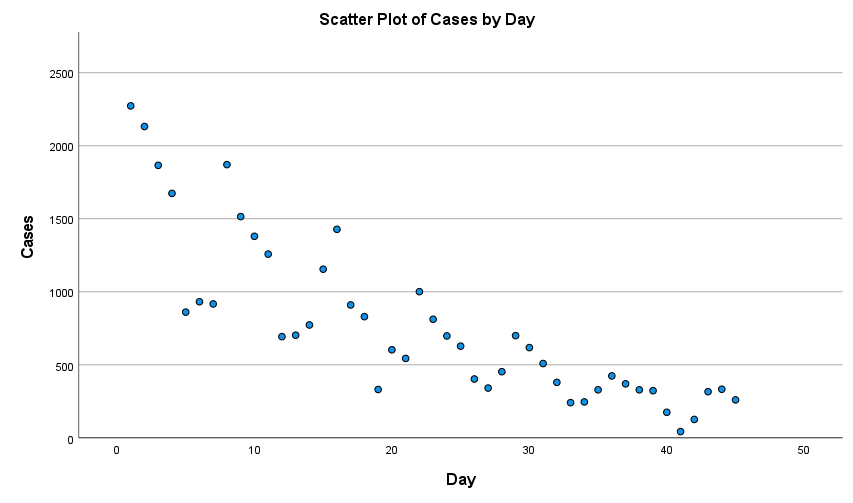
\includegraphics[width=1\textwidth,height=\textheight,keepaspectratio]{media/2/scatterplot_cases.png}
        	\end{subfigure}%
        \end{adjustbox}
        \caption{Διάγραμμα Διασποράς Ημερήσιων Κρουσμάτων στην Μολδαβία ως προς τον Αύξοντα Αριθμό Ημερών}
    \label{Moldova_cases}
    \end{figure}
    
    Παρατηρώντας το σχήμα φαίνεται να υπάρχει ισχυρή αρνητική γραμμική συσχέτιση μεταξύ των ημερήσιων θανάτων και του αύξοντα αριθμού ημέρας. Ο πίνακας \autoref{pearson_cases} επιβεβαιώνει τα παραπάνω.
    
    \begin{figure}[H]
        \centering
        \begin{adjustbox}{center}
        	\begin{subfigure}[c]{1\textwidth}    
        		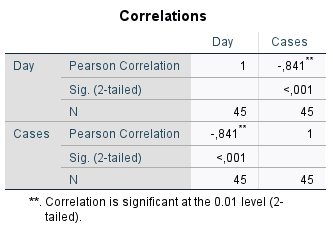
\includegraphics[width=1\textwidth,height=\textheight,keepaspectratio]{media/2/correlation_cases.png}
        	\end{subfigure}%
        \end{adjustbox}
        \caption{Συσχέτιση ημερήσιων θανάτων και αύξοντα Αριθμού Ημέρας στην Μολδαβία}
    \label{pearson_cases}
    \end{figure}
    
    \vfill
    
    Ο συντελεστής συσχέτισης \emph{\foreignlanguage{english}{Pearson}} που προκύπτει για το δείγμα Α είναι ίσος με -0.841, έχουμε δηλαδή όπως ειπώθηκε, ισχυρή αρνητική συσχέτιση για τα δεδομένα μας.
    
    Ακολουθούμε την ίδια διαδικασία για την εύρεση συσχέτισης, ή μη, μεταξύ των ημερήσιων θανάτων και του αύξοντα αριθμού ημερών. Το διάγραμμα διασποράς φαίνεται στο \autoref{deaths_scatter} και ο πίνακας για την εύρεση του συντελεστή συσχέτισης στο \autoref{pearson_deaths}.
    
    \vfill
    \newpage
    
     \begin{figure}[H]
        \centering
        \begin{adjustbox}{center}
        	\begin{subfigure}[c]{1\textwidth}    
        		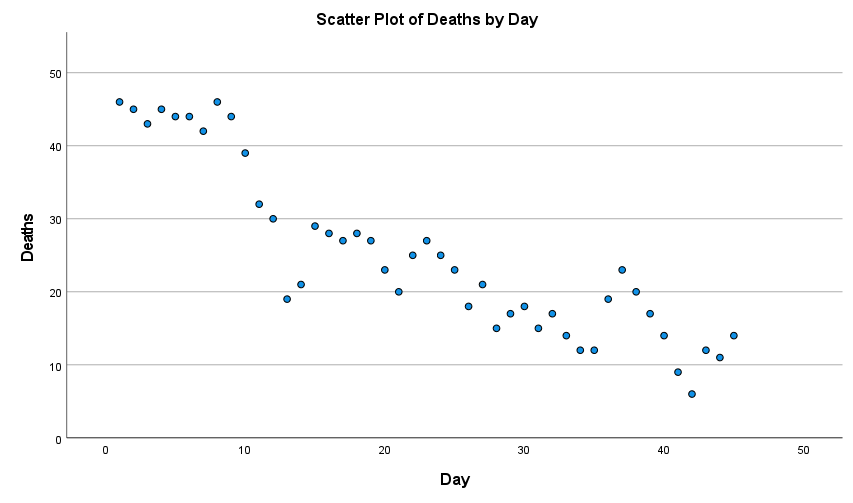
\includegraphics[width=1\textwidth,height=\textheight,keepaspectratio]{media/2/scatterplot_deaths.png}
        	\end{subfigure}%
        \end{adjustbox}
        \caption{Διάγραμμα Διασποράς Ημερήσιων Θανάτων στην Μολδαβία με τον Αύξοντα Αριθμό Ημέρας}
    \label{deaths_scatter}
    \end{figure}
    
    \begin{figure}[H]
        \centering
        \begin{adjustbox}{center}
        	\begin{subfigure}[c]{1\textwidth}    
        		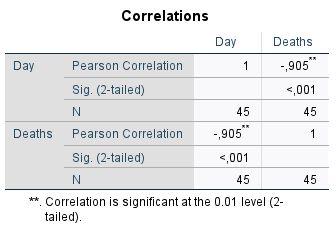
\includegraphics[width=1\textwidth,height=\textheight,keepaspectratio]{media/2/correlation_deaths.png}
        	\end{subfigure}%
        \end{adjustbox}
        \caption{Συσχέτιση Ημερήσιων Θανάτων και Αύξοντα Αριθμού Ημέρας στην Μολδαβία}
    \label{pearson_deaths}
    \end{figure}
    
    Και εδώ, υπάρχει αρνητική γραμική συχέτιση, όπως προκύπτεί από τα παραπάνω. Ο συντελεστής \emph{\foreignlanguage{english}{Pearson}} είναι ίσος με -0.905, δηλαδή και εδώ, έχουμε ισχυρή αρνητική συσχέτιση.
    
    
    \subsection{Μοντέλο Γραμμικής Παλινδρόμησης Ημερήσιων Κρουσμάτων και Θανάτων με τον Αύξοντα Αριθμό Ημέρας μετά την Κορύφωση του Κύματος}
    
    
    {\large \textbf{Ημερήσια Κρούσματα}}
    
    Για την εύρεση Μοντέλου Γραμμικής Παλινδρόμησης για τα ημερήσια κρούσματα χρησιμοποιούμε την μέθοδο ελαχίστων τετραγώνων και προκύπτει το \autoref{model_cases} και το  \autoref{coeff_cases}.
    
    \begin{figure}[H]
    \centering
    \begin{adjustbox}{center}
    	\begin{subfigure}[c]{1\textwidth}    
    		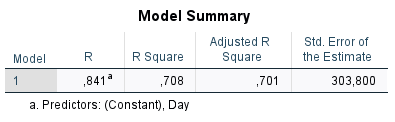
\includegraphics[width=1\textwidth,height=\textheight,keepaspectratio]{media/2/model_sum_cases.png}
    	\end{subfigure}%
    \end{adjustbox}
    \caption{Ισχύς Συσχέτισης των Δεδομένων για τα Ημερήσια Κρούσματα και τον Αύξοντα Αριθμό Ημέρας για την Μολδαβία}
    \label{model_cases}
    \end{figure}
    
    \begin{figure}[H]
    \centering
    \begin{adjustbox}{center}
    	\begin{subfigure}[c]{1\textwidth}    
    		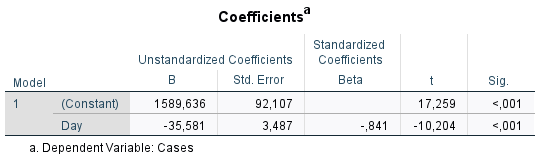
\includegraphics[width=1\textwidth,height=\textheight,keepaspectratio]{media/2/coeff_cases.png}
    	\end{subfigure}%
    \end{adjustbox}
    \caption{Συντελεστές γραμμικής Παλινδρόμησης για τα Ημερήσια Κρούσματα και τον Αύξοντα Αριθμό Ημέρας για την Μολδαβία}
    \label{coeff_cases}
    \end{figure}
    
    Όπως φαίνεται από τα παραπάνω, η εξίσωση γραμμικής παλινδρόμησης ισούται με:
    
    $ y = 1589.636 - 35.581x $ \\
    με τυπική  απόκλιση  σφαλμάτων  παλινδρόμησης ίση με 303.8
    Η γραμμική συσχέτιση σημειώνεται και στο \autoref{line_cases}.
    
    \begin{figure}[H]
    \centering
    \begin{adjustbox}{center}
    	\begin{subfigure}[c]{1\textwidth}    
    		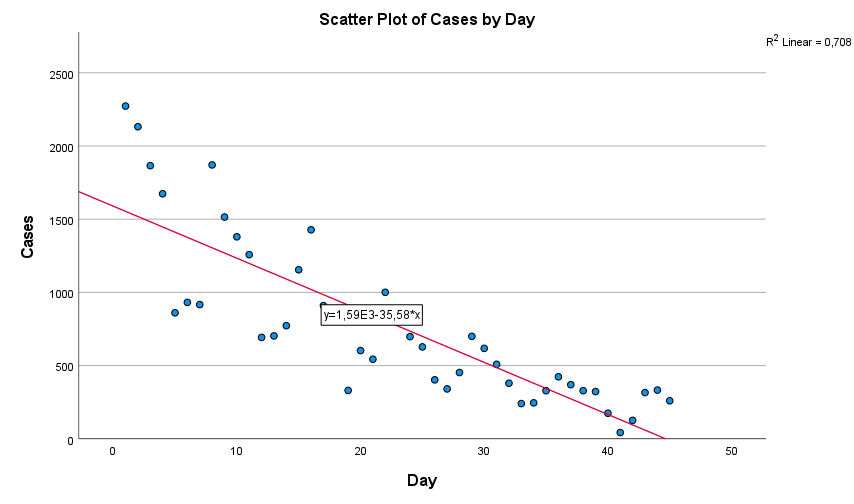
\includegraphics[width=1\textwidth,height=\textheight,keepaspectratio]{media/2/line_cases.png}
    	\end{subfigure}%
    \end{adjustbox}
    \caption{Η Ευθεία Παλινδρόμησης στο Διάγραμμα Διασποράς Κρουσμάτων για την Μολδαβία}
    \label{line_cases}
    \end{figure}
    
    \noindent
    {\large \textbf{Ημερήσιοι Θάνατοι}}
    \newline
     Όσον αφορά το Μοντέλο Γραμμικής Παλινδρόμησης ημερήσιων θανάτων ακολουθούμε την ίδια μεθοδολογία με τα προηγούμενα και προκύπτει το \autoref{model_deaths} και το  \autoref{coeff_deaths}.
     
     \begin{figure}[H]
    \centering
    \begin{adjustbox}{center}
    	\begin{subfigure}[c]{1\textwidth}    
    		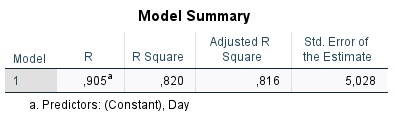
\includegraphics[width=1\textwidth,height=\textheight,keepaspectratio]{media/2/model_sum_deaths.png}
    	\end{subfigure}%
    \end{adjustbox}
    \caption{Ισχύς Συσχέτισης των Σεδομένων για τους Ημερήσιους Θανάτους με τον Αύξοντα Αριθμό Ημέρας στην Μολδαβία}
    \label{model_deaths}
    \end{figure}
    
    \begin{figure}[H]
    \centering
    \begin{adjustbox}{center}
    	\begin{subfigure}[c]{1\textwidth}    
    		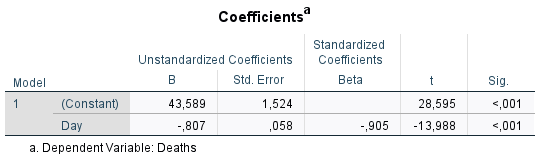
\includegraphics[width=1\textwidth,height=\textheight,keepaspectratio]{media/2/coeff_deaths.png}
    	\end{subfigure}%
    \end{adjustbox}
    \caption{Συντελεστές γραμμικής Παλινδρόμησης για τους ημερήσιους θανάτους με τον αύξοντα αριθμό ημέρας στην Μολδαβία}
    \label{coeff_deaths}
    \end{figure} 
    \noindent
   Aπό τα παραπάνω, η εξίσωση γραμμικής παλινδρόμησης ισούται με:
    
    $ y = 43.589 - 0.807x $ \\
    με τυπική  απόκλιση  σφαλμάτων  παλινδρόμησης ίση με 5.028
    Η γραμμική συσχέτιση σημειώνεται και στο \autoref{line_deaths}.
    
    \begin{figure}[H]
    \centering
    \begin{adjustbox}{center}
    	\begin{subfigure}[c]{1\textwidth}    
    		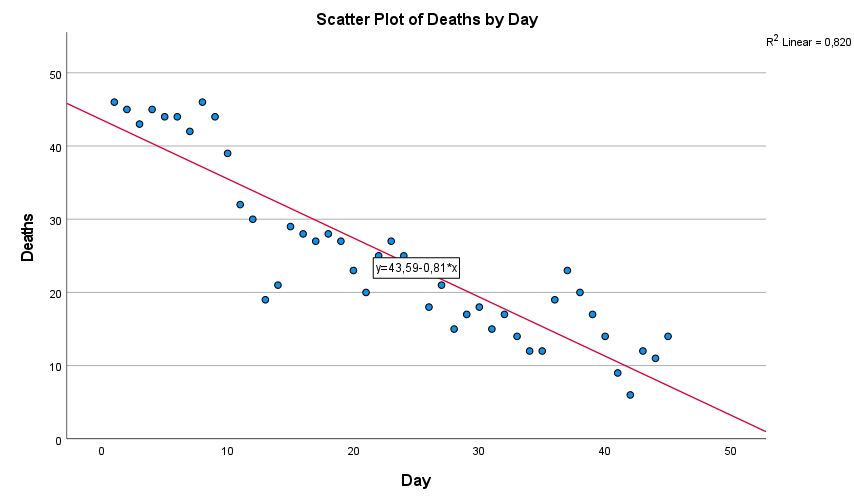
\includegraphics[width=1\textwidth,height=\textheight,keepaspectratio]{media/2/line_deaths.png}
    	\end{subfigure}%
    \end{adjustbox}
    \caption{Η Ευθεία Παλινδρόμησης στο Διάγραμμα Διασποράς Θανάτων για την Μολδαβία}
    \label{line_deaths}
    \end{figure}    

Είναι εμφανές, παρατηρώντας τα γραφήματα, ότι η σχέση μεταξύ κρουσμάτων και θανάτων με τον αύξοντα αριθμό ημέρας προσεγγίζουν την γραμμική συσχέτιση. Τα δύο μοντέλα είναι κατάλληλα για πρόβλεψη, καθώς εμφανίζουν μεγάλο συντελεστή $ R^2 $. Πρέπει, ωστόσο, να σημειωθεί ότι το μοντέλο πρόβλεψης θανάτων είναι καλύτερο από αυτό των κρουσμάτων λόγω της μικρότερης τυπικής  απόκλισης  σφαλμάτων παλινδρόμησης και του μεγαλύτερου συντελεστή $ R^2 $ 

\subsection{Πρόβλεψη Θανάτων κάποια Ημέρα \foreignlanguage{english}{t}, γνωρίζοντας τα Ημερήσια Κρούσματα τ Ημέρες Νωρίτερα}

\label{sec: guess_death}

\emph{Σε αυτό το εδάφιο θα δημιουργηθεί ένα μοντέλο πρόβλεψης, ώστε να μπορούν να προβλεφθούν οι ημερήσιοι θάνατοι, δεδομένου του αριθμού νέων κρουσμάτων \textbf{t} ημέρες πριν. Ως \textbf{t} ορίζουμε την χρονική υστέρηση που μεσολαβεί μεταξύ της κορύφωσης των ημερήσιων θανάτων και της κορύφωσης των ημερήσιων κρουσμάτων στο κύμα που μελετήσαμε στα προηγούμενα εδάφια.}

Χρησιμοποιούμε το δείγμα Α. Όπως ορίσαμε στην \autoref{sec:sample} το δείγμα Α, για την Μολδαβία περιλαμβάνει τις χρονικές περιόδους:
\begin{itemize}
    \item 24/03/2021 με 07/05/2021 για τα ημερήσια κρούσματα.
    \item 30/03/2021 με 13/05/2021 για τους ημερήσιους θανάτους.
\end{itemize}

Άρα ως ημέρες υστέρησης ορίζεται: $ \tau = $ 6 ημέρες.

Στο \autoref{line_deaths_cases} φαίνεται το διάγραμμα διασποράς μεταξύ των νέων θανάτων και νέων κρουσμάτων. Σημειώνεται και η ευθεία γραμμικής συσχέτισης που προκύπτει από την μέθοδο των ελαχίστων τετραγώνων. Η ανάλυση για την εύρεση της ευθείας γίνεται στην \autoref{sec:regression_t}. Στο \autoref{pearson_t6} φαίνεται και ο υπολογσιμός του συντελεστή \emph{\foreignlanguage{english}{Pearson}} ο οποίος προκύπτει ίσος με 0.866.

\begin{figure}[H]
    \centering
    \begin{adjustbox}{center}
    	\begin{subfigure}[c]{1\textwidth}    
    		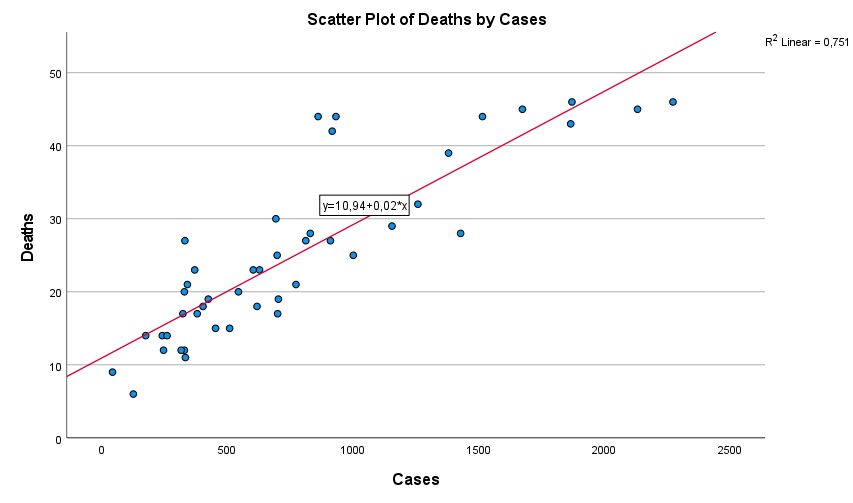
\includegraphics[width=1\textwidth,height=\textheight,keepaspectratio]{media/2/scatter_deaths_cases.png}
    	\end{subfigure}%
    \end{adjustbox}
    \caption{Διάγραμμα Διασποράς Ημερήσιων Θανάτων και Ημερήσιων Κρουσμάτων για την Μολδαβία}
    \label{line_deaths_cases}
\end{figure}

\begin{figure}[H]
    \centering
    \begin{adjustbox}{center}
    	\begin{subfigure}[c]{1\textwidth}    
    		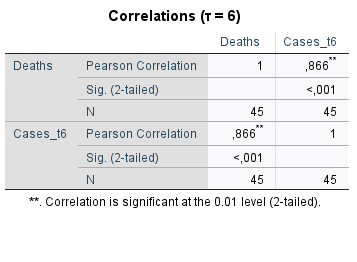
\includegraphics[width=1\textwidth,height=\textheight,keepaspectratio]{media/2/pearson_t6.png}
    	\end{subfigure}%
    \end{adjustbox}
    \caption{Συντελεστής \foreignlanguage{english}{Pearson} για $ \tau = 6 $}
    \label{pearson_t6}
\end{figure}

Ακολουθούμε την ίδια διαδικασία επιλέγοντας αυτή την φορά διαφορετικές τιμές για την υστέρηση $ \tau $, διατηρώντας σταθερά τα δεδομένα για τους θανάτους. Συγκεκριμένα θα επιλέξουμε $ \tau = 10 $ και $\tau = 20$. Με αυτά τα δεδομένα έχουμε:

\begin{itemize}
    \item για $ \tau = 10 $, προκύπτουν τα δεδομένα για τις ημέρες των κρουσμάτων κρουσμάτων: 20/03/2021 έως 03/05/2021.
    \item για $ \tau = 20 $, προκύπτουν τα δεδομένα για τις ημέρες των κρουσμάτων κρουσμάτων: 10/03/2021 έως 23/04/2021.
\end{itemize}

Στον \autoref{new_Moldova_data} παρατίθενται τα δεδομένα για τα ημερήσια κρούσματα για τις ημερομηνίες 10/03/2021 έως 23/03/2021, τα οποία δεν συμπεριλήφθηκαν στον \autoref{Moldova_data}

\begin{table}
    \centering
    \caption{Ημερήσια Κρούσματα Μολδαβίας για την Περίοδο 10/03/21 έως 23/03/21}
    \begin{tabular}{|l|l|}
    \hline
        Ημερομηνία & Ημ. Κρούσματα \\ \hline
        10-Μαρ-2021 & 873,00 \\ \hline
        11-Μαρ-2021 & 1896,00 \\ \hline
        12-Μαρ-2021 & 1785,00 \\ \hline
        13-Μαρ-2021 & 1801,00 \\ \hline
        14-Μαρ-2021 & 753,00 \\ \hline
        15-Μαρ-2021 & 861,00 \\ \hline
        16-Μαρ-2021 & 1688,00 \\ \hline
        17-Μαρ-2021 & 1916,00 \\ \hline
        18-Μαρ-2021 & 1797,00 \\ \hline
        19-Μαρ-2021 & 1843,00 \\ \hline
        20-Μαρ-2021 & 1635,00 \\ \hline
        21-Μαρ-2021 & 831,00 \\ \hline
        22-Μαρ-2021 & 1060,00 \\ \hline
        23-Μαρ-2021 & 1621,00 \\ \hline
    \end{tabular}
    \label{new_Moldova_data}
\end{table}

\begin{figure}
    \centering
    \begin{subfigure}[b]{0.8\textwidth}
        \centering
        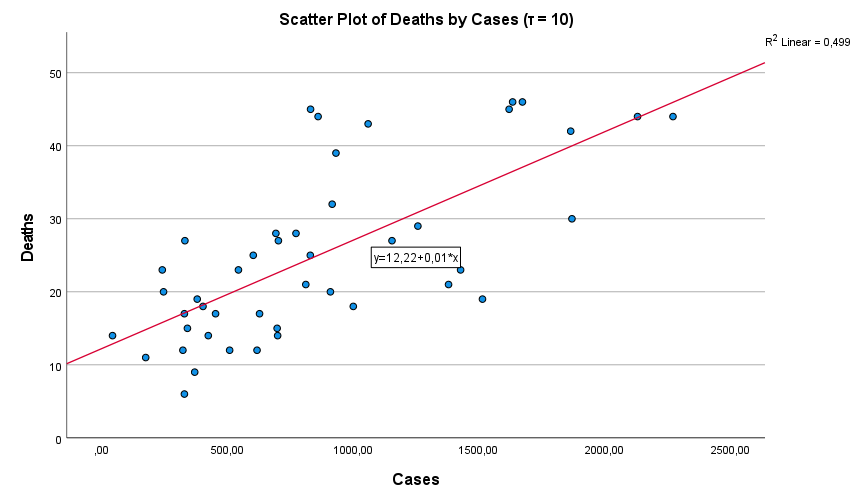
\includegraphics[width=\textwidth]{media/2/scatter_t10.png}
        \caption{Υστέρηση $ \tau = 10 $}    
    \end{subfigure} 
    \hfill
    \begin{subfigure}[b]{0.8\textwidth}  
        \centering 
        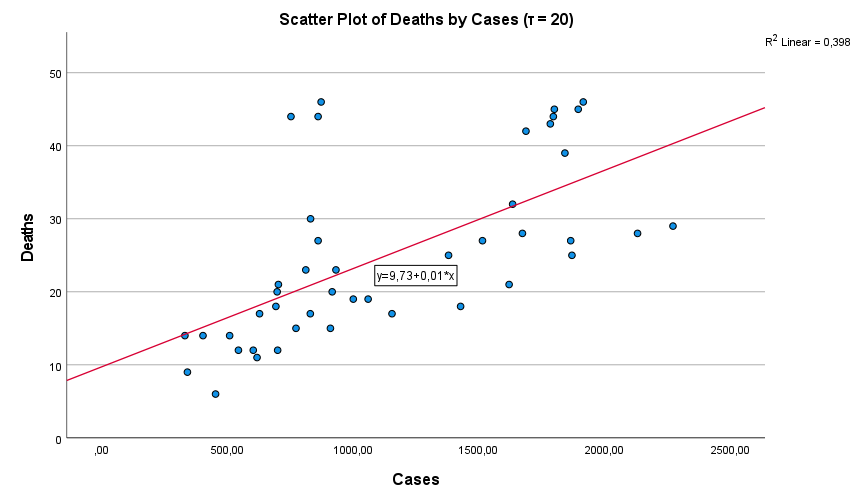
\includegraphics[width=\textwidth]{media/2/scatter_t20.png}
        \caption{Υστέρηση $ \tau = 20 $}    
    \end{subfigure}
    \caption{Γραφήματα Διασποράς για Διαφορετικές Τιμές Υστέρησης} 
    \label{scatter_t_10_20}
\end{figure}

Από την ανάλυση των δεδομένων για $ \tau = 10 $ και $ \tau = 20 $ πρoκύπτουν τα γραφήματα διασποράς στο \autoref{scatter_t_10_20}. Σημειώνεται και η ευθεία παλινδρόμησης που προκύπτει με την μέθοδο ελαχίστων τετραγώνων. Η ανάλυση για την εύρεση των ευθειών γίνεται και αυτή στην \autoref{sec:regression_t}. Ο συντελεστής \foreignlanguage{english}{Pearson} εμφανίζεται στο \autoref{pearson_t_10_20} και προκύπτει ίσος με 0.707 και 0.631 για τ = 10 και τ = 20 αντίστοιχα.

\begin{figure}
    \centering
    \begin{subfigure}[b]{0.8\textwidth}
        \centering
        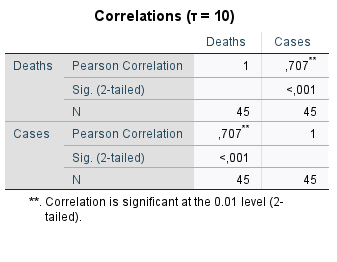
\includegraphics[width=\textwidth]{media/2/pearson_t10.png}
        \caption{τ = 10}     
    \end{subfigure} 
    \hfill
    \begin{subfigure}[b]{0.8\textwidth}  
        \centering 
        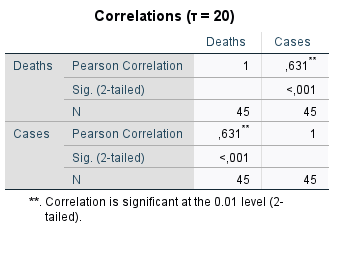
\includegraphics[width=\textwidth]{media/2/pearson_t20.png}
        \caption{τ=20}    
    \end{subfigure}
    \caption{Συντελεστής \foreignlanguage{english}{Pearson} για Διαφορετικές Τιμές του $ \tau $} 
    \label{pearson_t_10_20}
\end{figure}

Σε όλα τα γραφήματα φαίνεται καθαρά η θετική γραμμική σχέση που συνδέει τον αριθμό κρουσμάτων σε σχέση με τον μελλοντικό αριθμό θανάτων. Ωστόσο, θα πρέπει να σημειωθεί ότι η σχέση είναι ισχυρότερη όταν ως υστέρηση επιλέγεται η διαφορά της κορύφωσης ημερήσιων κρουσμάτων και ημερήσιων θανάτων ($ \tau = 6 $). Επίσης, πρέπει να σημειωθεί ότι η συσχέτιση για $ \tau = 10 $ είναι ισχυρότερη από την συσχέτιση για $ \tau = 20$. Αυτά ειναι προφανή από το σκόρπισμα που εμφανίζουν οι τιμές γύρω από την ευθεία παλινδρόμησης, και αποδεικνύονται με τον συντελεστή \foreignlanguage{english}{\emph{Pearson}}. 

\subsection{Εκτίμηση Μοντέλου Παλινδρόμησης για την εξάρτηση του αριθμού ημερήσιων νέων θανάτων από τον αριθμό των ημερήσιων νέων κρουσμάτων τ ημέρες}

\label{sec:regression_t}

\emph{Σε αυτό το εδάφιο θα εκτιμηθούν οι ευθείες που εμφανίζονται στα προηγούμενα διαγράμματα διασποράς και οι οποίες αποτελούν ένα μοντέλο πρόβλεψης των ημερήσιων θανάτων, βάσει των ημερήσιων κρυσμάτων που είχαμε $ \tau $ ημέρες νωρίτερα. Το $ \tau $, οπως και στην \autoref{sec: guess_death} ορίζεται ως 6 (Διαφορά κορύφωσης κύματος για κρούσματα και θανάτους), 10 και 20.}

Με την ανάλυση των δεδομένων για τις διάφορες τιμές του $ \tau $ προκύπτουν οι πίνακες που εμφανίζονται στο \autoref{reg_t_tables}

\begin{figure*}
        \centering
        \begin{subfigure}[b]{0.475\textwidth}
            \centering
            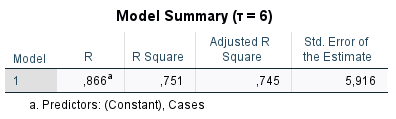
\includegraphics[width=\textwidth]{media/2/reg_t6_1.png}
        \end{subfigure}
        \hfill
        \begin{subfigure}[b]{0.475\textwidth}  
            \centering 
            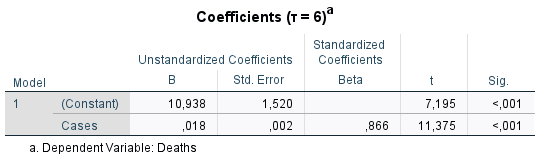
\includegraphics[width=\textwidth]{media/2/reg_t6_2.png}
        \end{subfigure}
        \vskip\baselineskip
        \begin{subfigure}[b]{0.475\textwidth}   
            \centering 
            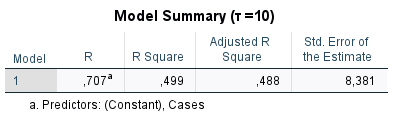
\includegraphics[width=\textwidth]{media/2/reg_t10_1.png}
        \end{subfigure}
        \hfill
        \begin{subfigure}[b]{0.475\textwidth}   
            \centering 
            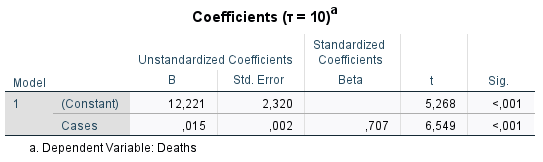
\includegraphics[width=\textwidth]{media/2/reg_t10_2.png}
        \end{subfigure}
        \begin{subfigure}[b]{0.475\textwidth}   
            \centering 
            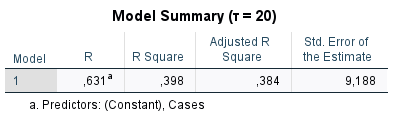
\includegraphics[width=\textwidth]{media/2/reg_t20_1.png}
        \end{subfigure}
        \hfill
        \begin{subfigure}[b]{0.475\textwidth}   
            \centering 
            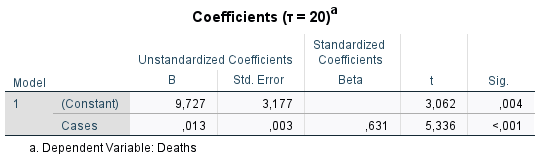
\includegraphics[width=\textwidth]{media/2/reg_t20_2.png}
        \end{subfigure}
        \caption{Ισχύς Παλινδρόμησης και Συντελεστές Παλινδρόμησης για τις διάφορες Τιμές του τ.}
        \label{reg_t_tables}
    \end{figure*}

    Προκύπτουν δηλαδή ότι προκύπτουν οι ευθείες:
    \begin{itemize}
        \item Για τ = 6: $ y = 10.938 + 0.018x $ με τυπική απόκλιση σφάλματος 5.916 και $ R^2 = 0.745 $
        \item Για τ = 10: $ y = 12.221 + 0.015x $ με τυπική απόκλιση σφάλματος 8.381 και $ R^2 = 0.488 $
        \item Για τ = 20: $ y = 9.727 + 0.13x $ με τυπική απόκλιση σφάλματος 9.188 και $ R^2 = 0.384 $
    \end{itemize}
    
    Eίναι εμφανές ότι καταλληλότερο μοντέλο πρόβλεψης είναι για χρόνο υστέρησης τ = 6, το οποίο έχει χαμηλότερη τυπική απόκλιση σφάλματος και υψηλότερο δείκτη $ R^2 $. Ακολουθεί το μοντέλο για τ = 10 και τέλος για τ = 20.
    
\newpage

\section{Παράρτημα}

\subsection{Κατάλογοι Σχημάτων και Πινάκων}

\listoffigures
\listoftables

\newpage

\section{Πηγές}

\begin{itemize}
    \item Όλα τα δεδομένα προέρχονται από το:
    
    \href{https://www.worldometers.info/coronavirus/}{\foreignlanguage{english}{https://www.worldometers.info/coronavirus/}}.
    \item Τα γραφήματα και οι πίνακες που παρατίθενται στο έγγραφο έγιναν με χρήση του λογισμικού \foreignlanguage{english}{\emph{IBM SPSS}}. 
    \item Για την συγγραφή χρησιμοποιήθηκε η γλώσσα δημιουργίας εγγράφων \LaTeX.
\end{itemize}
\end{document}